\documentclass[11pt]{article}
\usepackage{mypackages}
\begin{document}

% Max 

\section{Experiments and Expectations}

The aim of this project is to examine the effect of different amounts of threads
on the stability of deep reinforcement learning.
To acheive this we have solved both simple and advanced problems to investigate
the benefits and disadvantages of asynchronous training in two very different
settings.

\subsection{Solving CartPole using an Actor-Critic method with eligibility traces}

As a proof of concept we have implemented the method described in section
\ref{sec:actor_critic_el} for which the pseudo-code
can be found in appendix \ref{a:pseudo_code_et}.
The goal of this experiment is to show that a 
general/well-known/traditional/un-threaded Reinforcement Learning algorithm
is able to learn how to solve the CartPole problem, as well as provide a
baseline/minimum performance for the A3C algorithm.
[I.e as a test measure to check if A3C is performing at least as good
as the traditional/un-threaded Actor-Critic approach.]

For this experiments we used to separate neural networks, with no
shared weights, as policy and state-value estimators/parameterizations/approximators.
The network that approximates the state-value function consisted of an
input layer with four entries, corresponding to the format of a state in CartPole,
followed by a single hidden layer with eight neurons, and an output layer of a single
neuron.
We used a \textit{rectified linear unit} for activating the input to the
hidden layer and no/a linear activation for the output neuron.
% Her skal man enten skrive noget om RELU eller tilføje det i teori
For estimating the policy we used a network with the same structure,
with the only exception being that the output layer consisted of two
neurons, each corresponding to the probability of picking an action.
To emulate the probability distribution we used the softmax function
to activate the final layer.
[Måske noget om parametre her? jeg ved ikke helt hvordan man skal gøre
det for den her].

When we implemented the algorithm, we ran into some trouble with
the state-value estimator sometimes becoming too large, resulting
in both the probabilties and state-value estimates throwing a \texttt{NaN} error,
meaning they couldn't be represented using the bits they were assigned.
Therefore we have had to restrict the parameters of the algorithm to
be small when the used as a learning rate, which might cause the results of the
experiment being [unstable] and the method to learn at a slower pace
than can be achieved with a better implementation.

\subsection{Solving CartPole using the A3C algorithm}

To examine the effect of asynchronous training in a simpler setting than
that of the Atari games, we have implemented the A3C algorithm presented
in \cite{a3c} and given by the pseudo-code from appendix \ref{a:pseudo_code_a3c}.

We have chosen to also solve the CartPole problem with this approach as a way to
investigate if the usage of threaded training can increase the robustness
and stability of the algorithm, compared to the results of the more
traditional/simple/basic Actor-Critic approach as well as
to itself with different amounts of threads.

As in the previous implementation we ecnountered the \texttt{NaN} error,
but to a much lesser degree.
This means that the error should have little to no impact on
the final results.

To estimate the policy and state-value functions we will be using a single
neural network sharing a hidden layer.
The structure of the network resembles the structure used in the traditional/simple
Actor-Critic method, with the key difference being that the network has
two output layers

\begin{figure}[H]
    \centering
    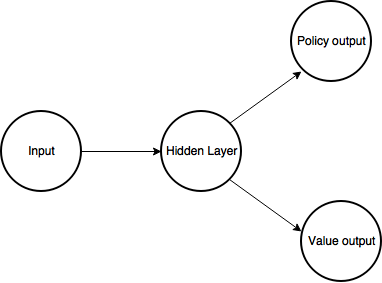
\includegraphics[scale=0.5]{include/shared_cartpole.png}
    \caption{The neural network used to estimate both the state-value
             and policy functions.}
    \label{fig:s_cartpole}
\end{figure}

For both the CartPole problem and the Atari games we will be using the same asynchronous setup
as described in \cite{a3c}.
This means that we will be using a single global network, whose only
purpose is to keep track of a set of global weights, and a local network
for each thread.
To perform the asynchronous update of the global weights we will be using
RMSpropagation as described in section \ref{sec:a3c}.
The parameters of the RMSpropagation, and the algorithm in general, have
been chosen because they provide decent test results.
Due to the time limitations of the project we haven't performed
a more sophisticated selection of the parameters, which might
influence the results of the experiments.

\subsection{Solving Atari Games}


\begin{figure}[H]
    \centering
    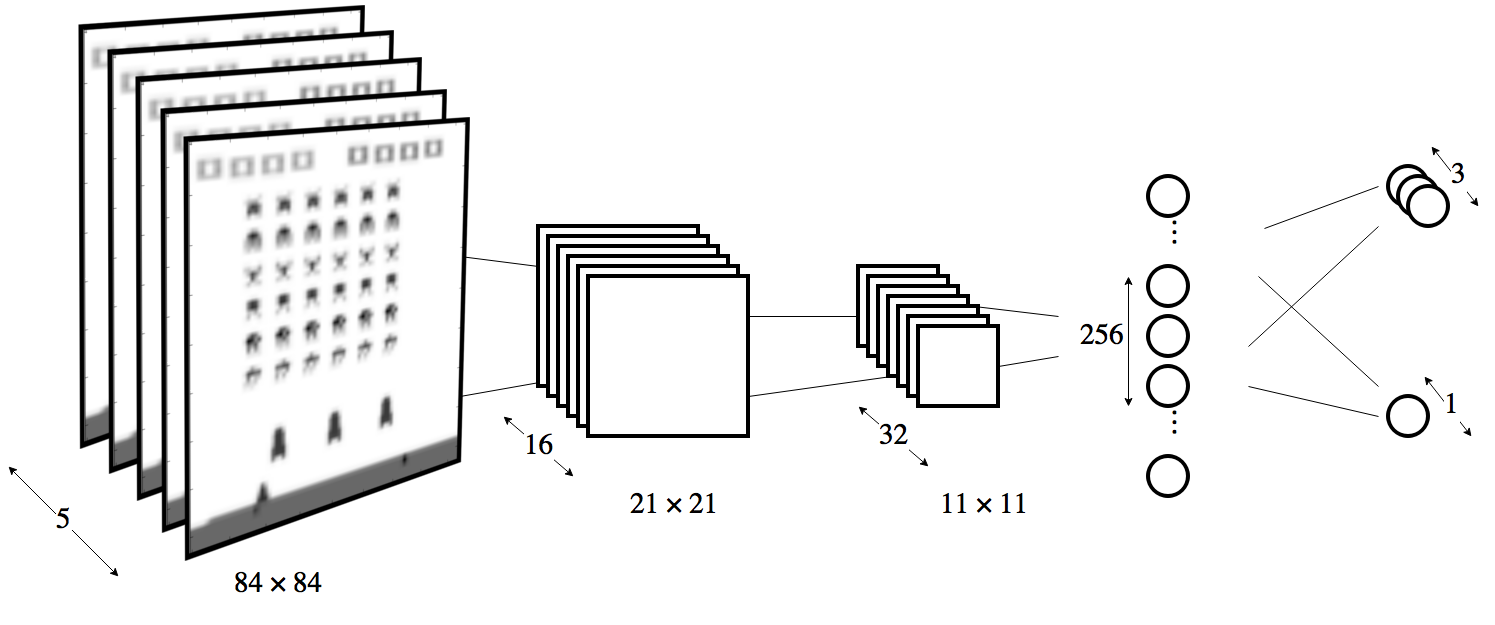
\includegraphics[scale=0.25]{include/Atari_network.png}
    \caption{The neural network used to estimate both the state-value
             and policy functions for Atari games. In this example the network
             is used on Space Invaders which means it has to assign each of three actions a probability.}
    \label{fig:atari_network}
\end{figure}

% Ramo
\section{Expectations and experiments}



The aim for this project is to use deep reinforcement learning for solving a simple reinforcement learning problem, analyze and discus the effect of different amounts of thread in asynchronous methods for deep reinforcement learning. For doing this we have set up some experiments. In section \ref{sec:improving_policies} we discussed how Actor-Critic algorithms works, and how to use eligibility traces combined with Actor-Critic. We have implemented the Actor-Critic algorithm using eligibilty traces, and for test our implementation we will use the CartPole problem discussed in section \ref{sec:Data}. We have also implemented the Advantage Actor-Critic methods discussed in section \ref{sec:a3c}, to test the implementation we using both the CartPole and the following Atari environments.

\subsection{Experimental Setup}

\subsubsection{Cartpole Actor-Critic using eligibilty traces}

The experiments performed on 


\subsubsection{Cartpole Advantage Actor-Critic (A3C)}


\subsubsection{Atari Advantage Actor-Critic (A3C)}

The experiments performed on the Atari games, used the following setup. Each experiments use either $1$, $2$, $4$, $8$ or $16$ local actors and $1$ global actor. Each local actor and the global one use the same neural network setup, with an input layer correspond to the input image after prepossessing discussed in section \ref{sec:atari}, then we use a convolutional layer with $16$ filters of size $8 \times 8$ with stride $4$, followed by a convolutional layer with $32$ filters of size $4 \times 4$ with stride $2$, then we have a dense layer using 256 units, all the 3 hidden layers use rectifier (ReLU) as activation function. We use this network for estimating both the state-value function and the policy, so after the hidden layers, we have two output layers one with a single output unit using a linear activation, representing the state action-value function. The other output layer have a output unit per available action in the problem and using softmax as activation, for present the probability of selecting an action, this output layer correspond to estimating the policy. All local actors updating the global weights after every 5 iterations using shared RMSProp for optimization, with a learning rate of $0.0001$, and a of $\alpha = 0.99$. For regularizing the influence the entropy have on the policy gradient, we mutiply the entorpy with $\beta = 0.01$. We also regularize the stepsize for the gradients of the state-value approximator by multipying with $\tau = 0.5$




\subsubsection{Atari Advantage Actor-Critic (A3C)}
\end{document}
